\section{遍历时间}
\label{sec:graph-walk-cover}

想象每到一个顶点就给它做上记号。走过已标记的顶点花了一步但没有新记号。遍历问题关心最后一个记号何时出现。

\subsection{遍历时间的计算}
\label{sec:graph-walk-cover-computation}

把起点计为已访问，定义\term{遍历时间}（cover time）$\tau_{\mathrm{cov}}$，分别记从$i$出发的遍历期望$C_i$和最坏起点的期望$C$，
\begin{equation}
\begin{aligned}
\tau_{\mathrm{cov}}&=\inf\{t\ge0:\{X_0,\ldots,X_t\}=V\},\\
C_i&=\mathbb{E}_i[\tau_{\mathrm{cov}}],
\qquad C=\max_i C_i.
\end{aligned}
\label{eq:graph-walk-cover-definition}
\end{equation}
遍历要求所有顶点都被访问，不要求每条边都经过。

\paragraph{完全图上的逐阶段收集}

在$K_n$的单位权游走中，若已经标记了$k$个顶点，当前顶点之外有$n-1$个等可能的去处，其中$n-k$个尚未标记。一步找到新顶点的概率为$p=(n-k)/(n-1)$。

只要这一步没有找到新顶点，记号数仍为$k$，下一步的情况完全一样。等待时间的期望$H$满足
\[
H=1+(1-p)H.
\]
式中$1$是必走的一步，$1-p$是失败后继续等$H$步。因此$H=1/p$。

将从$k$个记号增加到$k+1$个所需的平均步数$1/p=(n-1)/(n-k)$，按$k$从$1$到$n-1$相加。令$j=n-k$表示还未访问的顶点数，得到
\begin{equation}
C_i=(n-1)\sum_{j=1}^{n-1}\frac{1}{j}.
\label{eq:graph-walk-cover-complete}
\end{equation}
例如$K_4$的三段期望为$3/3=1$、$3/2$、$3/1=3$，合计$11/2$步。

\paragraph{路径端点的遍历}

在单位权$n$点路径上从端点$1$出发，首次到达另一端$n$之前必然经过所有中间顶点。因此$C_1=h_{1,n}$。两端之间串联了$n-1$条单位电阻边，$R_{1,n}=n-1$，总加权度$\operatorname{vol}(V)=2(n-1)$。路径反转后形状一样，所以$h_{1,n}=h_{n,1}$，由往返公式$2h_{1,n}=2(n-1)(n-1)$，得
\[
C_1=h_{1,n}=(n-1)^2.
\]
若起点在内部，遍历还需要覆盖两端，下一小节给出的统一上界可以处理任意起点。

\subsection{生成树上界}
\label{sec:graph-walk-cover-tree-bound}

一般图上很难直接按已访问集合分阶段计算，因为同样数量的记号可能分布在完全不同的区域。一种做法是：指定一份覆盖全图的访问次序，估计完成它所需的时间。由于实际遍历可能更早结束，这份次序给出的是遍历时间的上界。

以起点$u$为根取一棵生成树$T$，沿深度优先次序走完这棵树。每条树边去一次、回一次，沿途列出必须依次命中的目标。

例如四点环加对角线$\{1,3\}$，选择树路径$1\!-\!2\!-\!3\!-\!4$，从$1$出发的目标名单为$2,3,4,3,2,1$。这份名单只规定停止条件：先等到$2$、再等到$3$，以此类推。等待期间，棋子仍在原图上随机走，可以经过对角线。图~\ref{fig:graph-walk-cover-tree-targets}把所选的树和由它生成的名单放在一起。

\begin{BookInlineFigure}
\centering
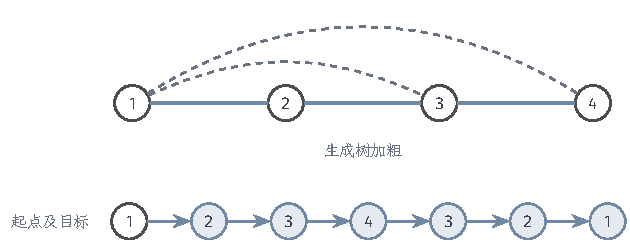
\includegraphics[width=106.726mm]{figures/03-graphs/05-matrices-and-spectra/tikz/walk-examples/cover-tree-targets.pdf}
\caption{用四点环加对角线$\{1,3\}$说明遍历上界。粗实线是所选树边，虚线是原图的其余边。下方从白底的起点$1$开始，箭头依次指向六个等待目标。实际游走仍可沿原图的所有边转移。}
\label{fig:graph-walk-cover-tree-targets}
\end{BookInlineFigure}

命中当前目标后，棋子的位置已经确定。下一段等待的期望就是从该位置出发的首达期望，与此前走过哪些顶点无关。

按名单完成全部目标时，每个顶点一定都已访问过。实际遍历可能更早结束——某些顶点在正式等到它之前已经顺路走过。因此名单给出的总等待时间是一个上界。

将每条树边的去程和返程配对，利用往返公式~\eqref{eq:graph-walk-commute-time}，得到
\begin{equation}
C_u\le\sum_{\{a,b\}\in T}(h_{a,b}+h_{b,a})
=\operatorname{vol}(V)\sum_{\{a,b\}\in T}R_{a,b}.
\label{eq:graph-walk-cover-resistance}
\end{equation}

每条树边$\{a,b\}$本身已经存在于图中。将全部单位电流送过这条边，可行流的耗散为$1/w_{a,b}$。有效电阻是所有单位流的最小耗散，因此$R_{a,b}\le1/w_{a,b}$。

对无权图，每条树边的$R_{a,b}\le1$，树有$n-1$条边，总加权度为$2m$，于是
\begin{equation}
C\le2m(n-1).
\label{eq:graph-walk-cover-unweighted}
\end{equation}
路径图的$m=n-1$，从端点出发的下界$(n-1)^2$与上界$2(n-1)(n-1)$同阶，因此最坏起点的遍历期望为$\Theta(n^2)$。

\paragraph{三次方量级的构造}

取一个$k$点完全图，在其中一个顶点$u$上接出一条含$\ell$条边的路径，末端为$v$。路径上所有边串联在$u,v$之间，完全图只在$u$处与路径相接，无法分担通往$v$的电流，因此$R_{u,v}=\ell$。

完全图已有$k(k-1)/2$条边，路径增加$\ell$条，每条边两端都计入度数，总加权度为$k(k-1)+2\ell$。

从$v$出发首次到达$u$以前，棋子只能在路径上行走，故$h_{v,u}=\ell^2$。利用往返公式减去这一方向，得
\[
h_{u,v}=\operatorname{vol}(V)\,R_{u,v}-h_{v,u}
=(k(k-1)+2\ell)\ell-\ell^2=k(k-1)\ell+\ell^2.
\]
遍历至少要到达$v$。当$k$与$\ell$都和$n=k+\ell$同阶时，这一项给出$\Theta(n^3)$的下界，与式~\eqref{eq:graph-walk-cover-unweighted}的上界量级一致。大量边集中在一个团里，增加了找到路径入口前的等待。
